\documentclass[11pt]{article}
\usepackage[margin=1in]{geometry}
\usepackage{amsmath,amssymb}
\usepackage{graphicx}
\usepackage{hyperref}
\usepackage{booktabs}

\newcommand{\Msun}{M_\odot}
\newcommand{\lcdm}{\Lambda\text{CDM}}

\title{$M_\mathrm{enc}(r_{1/2})$ Distributions from Modified Power Spectra}
\author{Adrienne L. Erickcek}
\date{\today}

\begin{document}
\maketitle

\section{Overview}

This note describes the MassEncCDF.py pipeline that computes how modifications to the
primordial matter power spectrum propagate through the halo mass function,
concentration--mass relation, and NFW density profiles to produce
observable differences in the enclosed mass within the stellar half-light
radius, $M_{\rm enc}(r_{1/2})$.  This code is adapted from a Jupyter notebook that Daniel Gilman wrote during the Spec-S5 dark matter workshop in March 2026. 

Four beyond-$\lcdm$ scenarios are
compared to a Planck~2018 $\lcdm$ reference:

\begin{itemize}
  \item \textbf{WDM} --- a warm dark matter--like cutoff,
        $P(k)\to P_{\lcdm}(k)\,[1+(k/k_{\rm cut})^\nu]^{-5/\nu}$
        with $k_{\rm cut}=150\;h/$Mpc and $\nu=1.12$.
  \item \textbf{vEDE} --- a very early dark energy (vEDE) model \cite{vEDE}
        with parameters $\mathcal{R}=60$ and $\log_{10}a_c=-6.92$
        (see Figure~9 of that paper), with all other parameters held at
        their Planck~2018 values.
  \item \textbf{AK1} --- the fiducial two-field axion-kination model
        \cite{AK1} (Figure~12 of that paper), whose $P(k)$ is provided
        as numerical arrays together with a $\lcdm$ reference so that
        $T(k)=\sqrt{P(k)/P_{\rm ref}(k)}$ can be applied to the
        Planck~2018 spectrum.
  \item \textbf{CDM} --- the $\lcdm$ baseline (Planck~2018 cosmology).
\end{itemize}

All cosmological computations (power spectra, $\sigma(M)$, mass
functions, and concentrations) use the \textsc{Colossus} toolkit with the
Planck~2018 parameter set \cite{Diemer:2017bwl}.

\section{Power Spectra and Variance}

The code begins with the Planck~2018 $\lcdm$ linear matter power
spectrum $P_{\lcdm}(k)$ tabulated on a grid of 3000 points uniformly
spaced in $\log_{10} k$ from $10^{-5}$ to $10^{3.7}\;h/$Mpc.  Each
beyond-$\lcdm$ model modifies this spectrum through a transfer function,
\begin{equation}
  P_X(k) = T_X^2(k)\,P_{\lcdm}(k)\,,
\end{equation}
where $T_X(k)$ depends on the model.  The variance of the linear density
field smoothed on scale $R$ is
\begin{equation}
  \sigma^2(R) = \frac{1}{2\pi^2}\int_0^\infty k^2\,P(k)\,
  |\tilde{W}(kR)|^2\,dk\,,
\end{equation}
with $R$ the Lagrangian radius corresponding to halo mass $M$ via
$M = (4\pi/3)\,\bar\rho\,R^3$.

Figure~\ref{fig:pk} shows the four power spectra and
Figure~\ref{fig:sigma} shows the resulting $\sigma(M)$.

\begin{figure}[htbp]
  \centering
  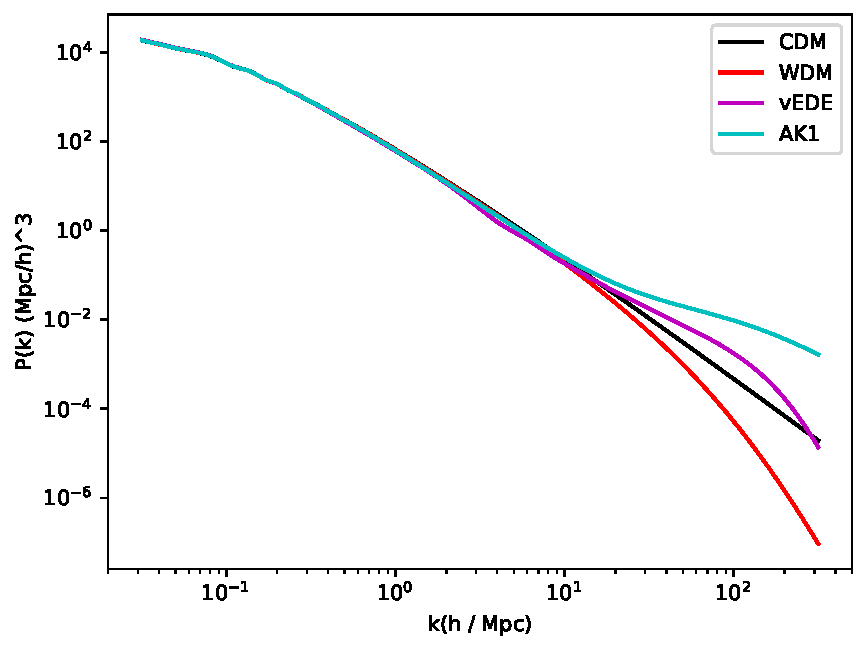
\includegraphics[width=0.7\textwidth]{power_spectrum.pdf}
  \caption{Linear matter power spectra for each model.}
  \label{fig:pk}
\end{figure}

\begin{figure}[htbp]
  \centering
  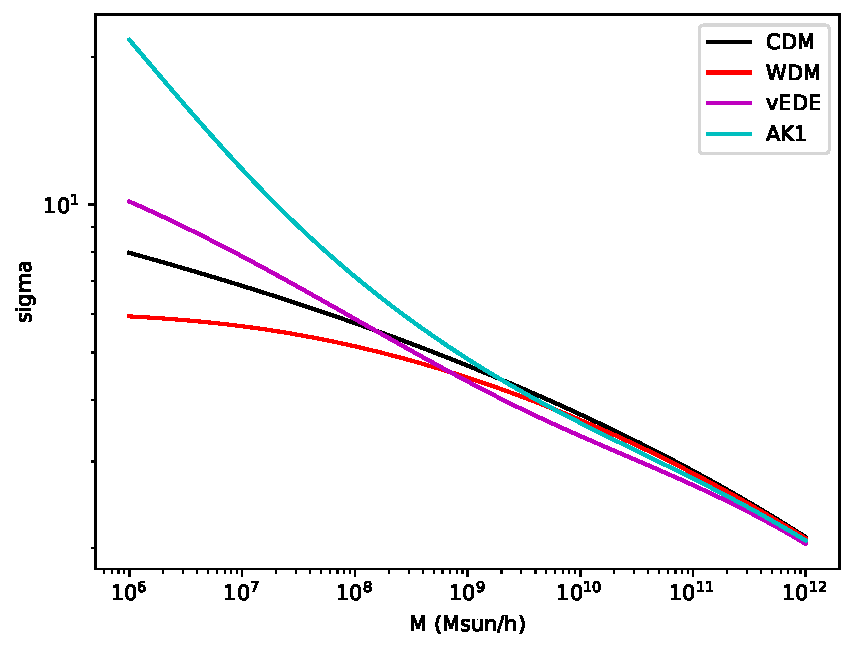
\includegraphics[width=0.7\textwidth]{sigma_M.pdf}
  \caption{RMS density fluctuation $\sigma(M)$ as a function of halo
  mass for each model.}
  \label{fig:sigma}
\end{figure}

\section{Concentration--Mass Relation}

Halo concentrations are computed using the Diemer \& Joyce 2019 \cite{Diemer19} model as
implemented in \textsc{Colossus}, evaluated at $z=0$ for each modified
power spectrum.  The resulting concentration--mass relations are shown in
Figure~\ref{fig:cm}.

\begin{figure}[htbp]
  \centering
  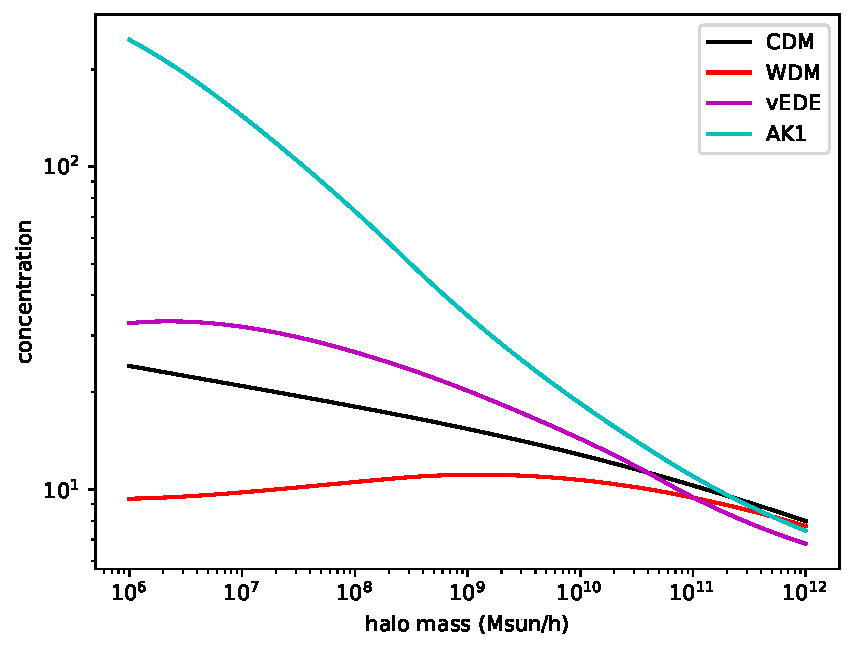
\includegraphics[width=0.7\textwidth]{concentration_mass.pdf}
  \caption{Concentration--mass relation $c(M)$ at $z=0$ for each model.}
  \label{fig:cm}
\end{figure}

\section{Halo Mass Function}

The halo mass function $dn/d\ln M$ is evaluated at $z=0$ on a grid of 50
masses uniformly spaced in $\log_{10} M$ from $10^{6}$ to
$10^{12}\;\Msun/h$, using the \textsc{Colossus}
\texttt{massFunction} routine with each model's custom power spectrum
(Figure~\ref{fig:mf}).

\begin{figure}[htbp]
  \centering
  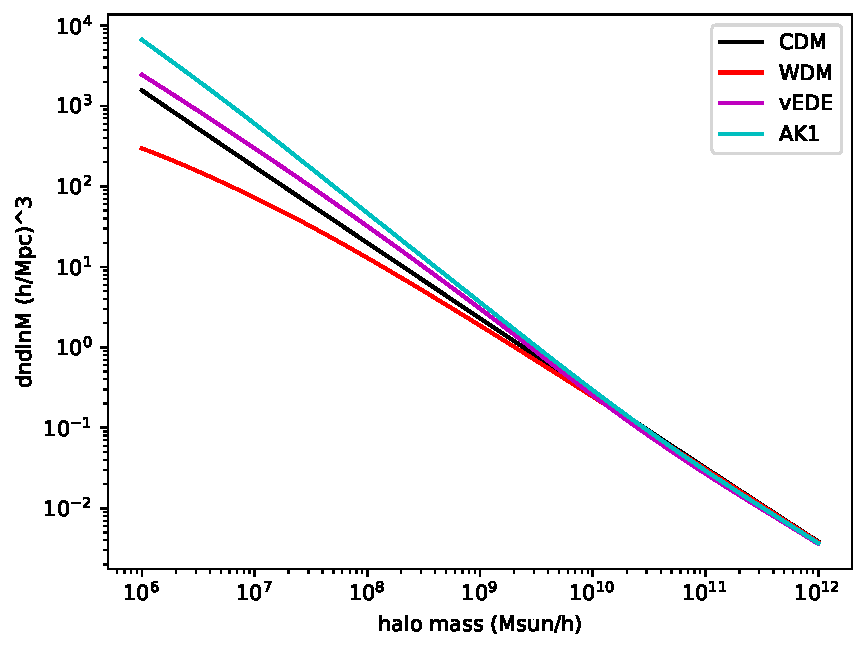
\includegraphics[width=0.7\textwidth]{mass_function.pdf}
  \caption{Halo mass function $dn/d\ln M$ at $z=0$ for each model.}
  \label{fig:mf}
\end{figure}

\section{Monte Carlo Sampling}
\label{sec:sampling}

To generate mock halo populations we draw masses from each mass function
via inverse-CDF sampling.  The procedure is:

\begin{enumerate}
  \item \textbf{Build the CDF.}  Given the tabulated
    $f_i \equiv (dn/d\ln M)_i$ on the $\log_{10}M$ grid, define
    trapezoidal bin weights
    \begin{equation}
      w_i = \tfrac{1}{2}\bigl(f_i + f_{i+1}\bigr),
      \qquad i=0,\dots,N{-}2\,,
    \end{equation}
    and set $\text{CDF}_0=0$,\;
    $\text{CDF}_j=\sum_{i=0}^{j-1}w_i$ for $j=1,\dots,N{-}1$.
    Because the grid spacing $\Delta\!\log_{10}M$ is constant it cancels
    after dividing by $\text{CDF}_{N-1}$, leaving a properly normalized
    CDF.

  \item \textbf{Invert.}  Construct a 1-D interpolant
    $\text{CDF}\to\log_{10}M$.  Draw $N_{\rm draw}$ uniform random
    variates $u\in[0,1]$ and compute
    $M = 10^{\,\text{CDF}^{-1}(u)}$.

  \item \textbf{Scale the number of draws.}  The CDF is normalized to
    unity regardless of the overall amplitude of the mass function, so
    the number of draws must encode the relative abundance of halos
    across models.  We set
    \begin{equation}
      N_{{\rm draw},X}
        = N_{{\rm draw,CDM}}
          \times \frac{\int (dn/d\ln M)_X\,d\!\log_{10}M}
                      {\int (dn/d\ln M)_{\rm CDM}\,d\!\log_{10}M}\,.
      \label{eq:scale}
    \end{equation}
    The common factor of $\ln 10$ that converts
    $d\!\log_{10}M\to d\!\ln M$ cancels in the ratio, so integrating
    over $\log_{10}M$ is sufficient.  Both the numerator and denominator
    are evaluated with \texttt{np.trapz}, matching the trapezoidal rule
    used for the CDF.
\end{enumerate}

Figure~\ref{fig:sampled} shows a histogram of the sampled masses for a
diagnostic run with $5\times10^{7}$ reference draws.

\begin{figure}[htbp]
  \centering
  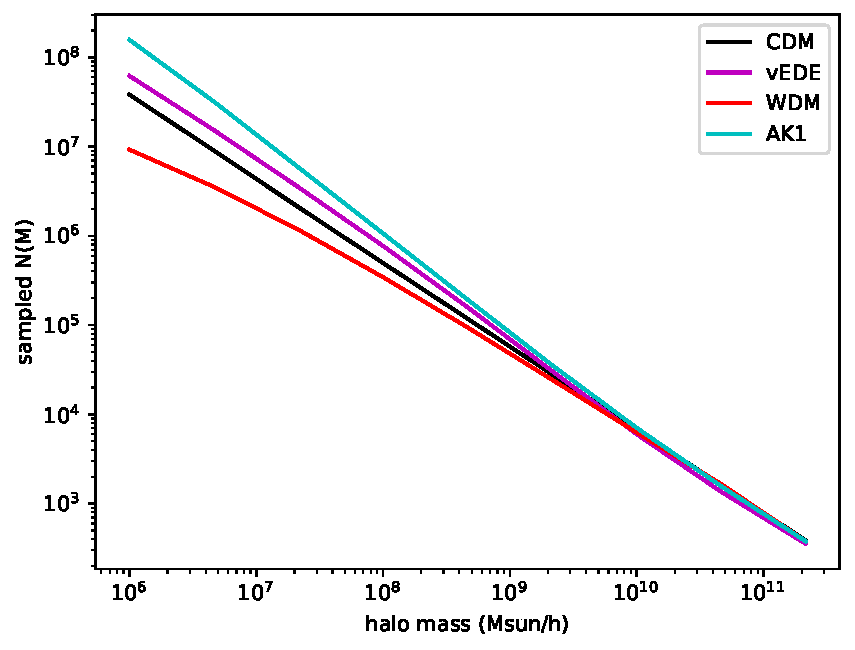
\includegraphics[width=0.7\textwidth]{sampled_mass_distribution.pdf}
  \caption{Histogram of halo masses drawn from each model's mass
  function, confirming that the sampling reproduces the correct relative
  abundances.}
  \label{fig:sampled}
\end{figure}

\section{NFW Enclosed Mass within Stellar Half-light Radius}

For each sampled halo of mass $M$ the pipeline:
\begin{enumerate}
  \item Assigns a concentration $c$ by interpolating the tabulated
    $c(M)$ relation and adding lognormal scatter with
    $\sigma_{\ln c}=0.15$.
  \item Computes a stellar half-light radius
    $r_{1/2}=0.040\,(r_{\rm vir}/10\;\text{kpc})$\,kpc \cite{Nadler20}
    with lognormal scatter $\sigma_{\ln r_{1/2}}=0.6$.
  \item Evaluates the NFW enclosed mass
    \begin{equation}
      M_{\rm enc}(r_{1/2})
        = 4\pi\,\rho_s\,r_s^3
          \left[\ln\!\left(1+\frac{r_{1/2}}{r_s}\right)
                - \frac{r_{1/2}/r_s}{1+r_{1/2}/r_s}\right],
    \end{equation}
    where $\rho_s$ and $r_s$ are the NFW scale density and scale radius
    obtained from $(M,c)$ via \textsc{Colossus}.
\end{enumerate}

Halos below $M_{\rm min}=10^{8}\;\Msun/h$ or with
$r_{1/2}<0.01$\,kpc are discarded.  The final production run uses
$10^{8}$ reference CDM draws (scaled per Eq.~\ref{eq:scale} for the
other models).  Figure~\ref{fig:scatter} shows the resulting
$M_{\rm enc}/M$ versus $r_{1/2}$ scatter plot for a randomly selected subset of the sample.

\begin{figure}[htbp]
  \centering
  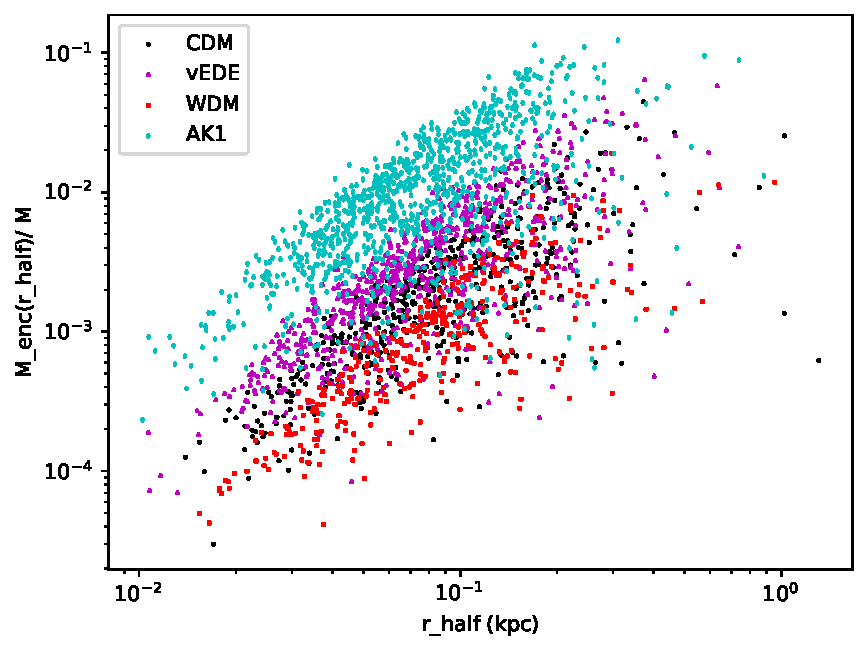
\includegraphics[width=0.7\textwidth]{menc_vs_rhalf.pdf}
  \caption{Enclosed mass fraction $M_{\rm enc}(r_{1/2})/M$ versus
  half-light radius for a random subsample of halos in each model.}
  \label{fig:scatter}
\end{figure}

\section{Complementary CDF of Enclosed Mass}

The main observable is the complementary cumulative distribution function
(CCDF) of $M_{\rm enc}(r_{1/2})$. This is computed in 50 logarithmically spaced bins from $10^{4}$ to
$10^{10}\;\Msun$.  Because the number of draws is scaled by the
mass-function integral ratio (Eq.~\ref{eq:scale}), differences between
models in $N(>M_{\rm enc})$ directly reflect the physical differences in
halo abundance and internal structure.  The result is shown in
Figure~\ref{fig:cdf}. 

\begin{figure}[htbp]
  \centering
  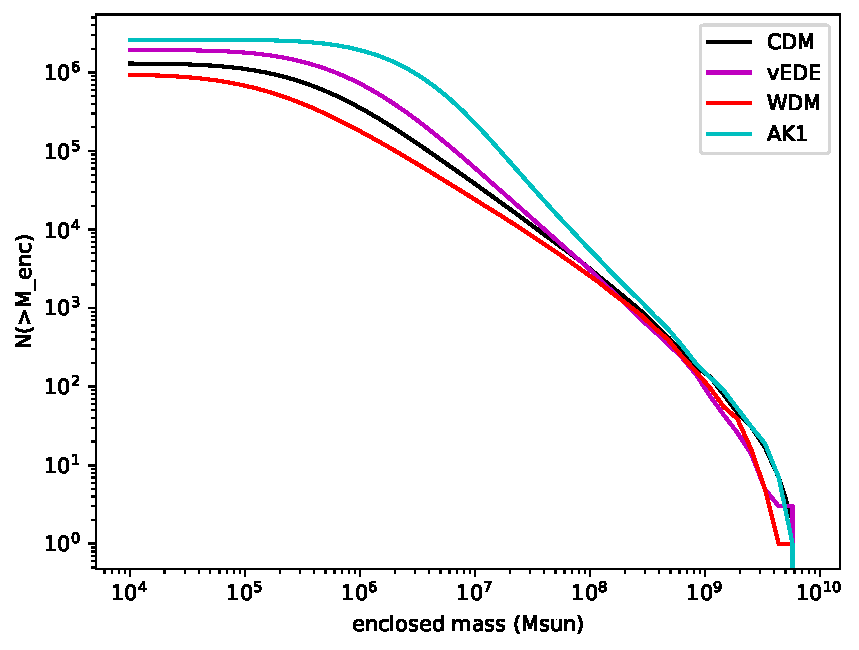
\includegraphics[width=0.7\textwidth]{menc_cdf.pdf}
  \caption{Complementary CDF of the enclosed mass $M_{\rm enc}(r_{1/2})$
  for each model based on a sample of halos with $M>10^{8}\;\Msun/h$ and 
 $r_{1/2}>0.01$\,kpc. The halo sample for each power spectrum has the same $N(M)$ for $M\gtrsim10^{10} \Msun/h$, 
  as seen in Fig.~\ref{fig:sampled}. Differences between curves indicate the observable
  impact of modified power spectra on subhalo populations.}
  \label{fig:cdf}
\end{figure}

\begin{thebibliography}{9}
\bibitem{vEDE}
A.~C.~Sobotka, A.~L.~Erickcek and T.~L.~Smith,
``Signatures of very early dark energy in the matter power spectrum,''
Phys. Rev. D \textbf{111}, no.12, 123522 (2025)
doi:10.1103/9bd9-fzwh
[arXiv:2409.06778 [astro-ph.CO]].

\bibitem{AK1}
R.~T.~Co, N.~Fernandez, A.~Ghalsasi, K.~Harigaya and J.~Shelton,
%``Enhanced matter power spectrum from axion kination after Big Bang nucleosynthesis,''
JCAP \textbf{02}, 082 (2026)
doi:10.1088/1475-7516/2026/02/082
[arXiv:2510.01308 [hep-ph]].

%\cite{Diemer:2017bwl}
\bibitem{Diemer:2017bwl}
B.~Diemer,
%``COLOSSUS: A python toolkit for cosmology, large-scale structure, and dark matter halos,''
Astrophys. J. Suppl. \textbf{239}, no.2, 35 (2018)
doi:10.3847/1538-4365/aaee8c
[arXiv:1712.04512 [astro-ph.CO]].

\bibitem{Diemer19}
 B.~Diemer and M.~Joyce,
%``An accurate physical model for halo concentrations,''
Astrophys. J. \textbf{871}, no.2, 168 (2019)
doi:10.3847/1538-4357/aafad6
[arXiv:1809.07326 [astro-ph.CO]].

\bibitem{Nadler20}
E.~O.~Nadler \textit{et al.} [DES],
%``Milky Way Satellite Census -- II. Galaxy-Halo Connection Constraints Including the Impact of the Large Magellanic Cloud,''
Astrophys. J. \textbf{893}, 48 (2020)
doi:10.3847/1538-4357/ab846a
[arXiv:1912.03303 [astro-ph.GA]].
\end{thebibliography}



\end{document}
